\documentclass[crop]{standalone}

\usepackage[dvipsnames]{xcolor}
\usepackage{tikz}

\usetikzlibrary{backgrounds}

\begin{document}
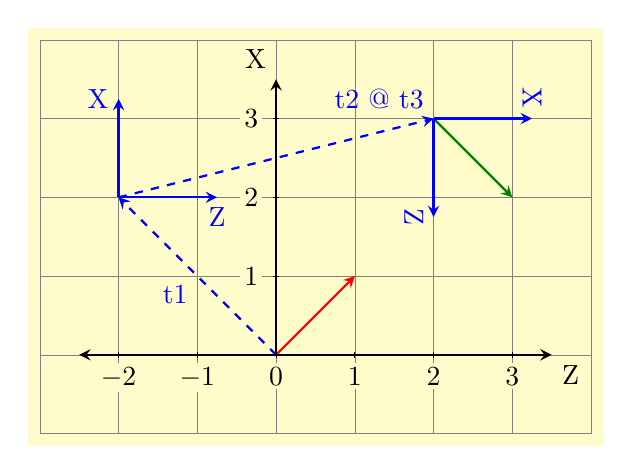
\begin{tikzpicture}[background rectangle/.style={fill=yellow!20}, show background rectangle]


	\draw[step=1cm,gray,very thin] (-3,-1) grid (4,4);

	\foreach \z in {-2,-1,0,1,2,3}
		\draw (\z cm,1pt) -- (\z cm,-1pt) node[anchor=north, inner sep=1.5pt, outer ysep=2pt, fill=yellow!20] {$\z$};
	\foreach \x in {1,2,3}
		\draw (1pt,\x cm) -- (-1pt,\x cm) node[anchor=east, inner sep=1.5pt, outer xsep=4pt, fill=yellow!20] {$\x$};

	\draw[thick,-stealth,red] (0,0) -- (1,1);
	\draw[thick,-stealth,blue,dashed] (0,0) -- (-2,2);
	\node[blue,anchor=north east] at (-1,1) {t1};
	\draw[thick,-stealth,blue,dashed] (-2,2) -- (2,3);
	\node[blue,anchor=south east] at (2,3) {t2 @ t3};
	\begin{scope}[shift={(2,3)},rotate=-90,transform shape]
		\draw[thick,-stealth,Green] (0,0) -- (1,1);
	\end{scope}

	\begin{scope}[shift={(-2,2)},blue,transform shape]
		\draw[thick,-stealth] (0,0) -- (1.25,0) node[anchor=north] {Z};
		\draw[thick,-stealth] (0,0) -- (0,1.25) node[anchor=east] {X};
	\end{scope}

	\begin{scope}[shift={(2,3)},rotate=-90,blue,transform shape]
		\draw[thick,-stealth] (0,0) -- (1.25,0) node[anchor=north] {Z};
		\draw[thick,-stealth] (0,0) -- (0,1.25) node[anchor=east] {X};
	\end{scope}

	\draw[thick,stealth-stealth] (-2.5,0) -- (3.5,0) node[anchor=north west] {Z};
	\draw[thick,-stealth] (0,0) -- (0,3.5) node[anchor=south east] {X};


\end{tikzpicture}
\end{document}
